\loai{Loại 1: Tính Q của 1 vật}
\begin{ex}
	 Biết nhiệt dung riêng của nhôm là $880 \ J / kg . K$. Nhiệt lượng cần thiết để tăng nhiệt độ của một miếng nhôm có khối lượng $810 \ g$ từ $20^\circ C$ đến $75^\circ C$ là
	\choice
	{39804 J}
	{\True 39204 J}
	{36204 J}
	{38704 J}
	\loigiai{
		Nhiệt lượng cần thiết:  $Q=mc\Delta t=39204 \ J$.
	}
	\haidong{6}\end{ex}
\begin{ex} \nguon{2}
	Biết nhiệt độ ban đầu của nước là $20^\circ C$ và nhiệt dung riêng của nước là $4200 \ J / kg . K$. Để đun sôi 15 kg nước ở áp suất 1 atm cần cung cấp một nhiệt lượng là 
	\choice
	{\True $5040 \ k J$}
	{$5040 \ J$}
	{$50,40 \ k J$}
	{$5,040 \ J$}
	
	\loigiai{
		
		\begin{itemize}
			\item Khối lượng của nước: $m = 15 \ kg$ (vì 1 lít nước tương đương 1 kg)
			\item Nước cần tăng nhiệt độ từ $20^\circ C$ lên $100^\circ C$, chênh lệch nhiệt độ $\Delta t = 80^\circ C$
			\item Nhiệt lượng cần thiết:
			$$Q = mc\Delta t = 15 . 4200 . 80 = 5040000 \ J = 5040 \ kJ$$
		\end{itemize}
	}
\end{ex}



\loai{Loại 2: Tính Q của 1 vật - bài toán ngược}


\begin{ex} \nguon{3}
	$100\ g$ chì khi được truyền nhiệt lượng $260\ J$  thì tăng nhiệt độ từ $15^\circ C$ đến $35^\circ C$. Nhiệt dung riêng của chì là
	\choice
	{\True $130\ J/kg . K$}
	{$26\ J/kg . K$}
	{$130\ kJ/kg . K$}
	{$260\ kJ/kg . K$}
	\loigiai{
		$Q=mc \Delta t \Rightarrow c=\dfrac{Q}{m \Delta t}=\dfrac{260}{0,1 .(35-15)}=130\ J/kg.K \Rightarrow$ Chọn A
	}
\end{ex}

\loai{Loại 3: Tính Q theo P của 1 vật}
\begin{ex}
	Người ta thực hiện thí nghiệm xác định nhiệt dung riêng của đồng với một miếng đồng có khối lượng 850 g. Lúc đầu nhiệt độ của miếng đồng là $12^\circ C$. Thời gian từ khi bật bộ phận đốt nóng có công suất 40 W đến khi nhiệt độ của miếng đồng tăng tới $30^\circ C$ là 146 giây. Giả sử toàn bộ nhiệt lượng được dùng để làm tăng nhiệt độ của miếng đồng. Nhiệt dung riêng của đồng được xác định có giá trị là
	\choice
	{\True $381,7\ J/kg.K$}
	{$391,7\ J/kg.K$}
	{$401,7\ J/kg.K$}
	{$281,7\ J/kg.K$}
	\loigiai{
		\begin{itemize}
			\item Nhiệt dung riêng của đồng: $c=\dfrac{Q}{m\Delta t}=\dfrac{Pt}{m\Delta t}=\dfrac{40.146}{0,85.(30-12)}=381,7\ J/kg.K$.
		\end{itemize}
	}
	\haidong{8}\end{ex}









\begin{ex} \nguon{2}
	Một ấm nhôm có khối lượng $300 \ g$ chứa 0,5 lít nước đang ở nhiệt độ $25^\circ C$. Biết khối lượng riêng của nước là $1000\ kg/m^3$; nhiệt dung riêng của nhôm, nước lần lượt là $c_1=880 \ J / kg . K,\ c_2=4200 \ J / kg . K$. Nhiệt lượng cần cung cấp để đun sôi nước trong ấm ở áp suất 1 atm là
	\choice
	{\True $177,3 \ kJ$}
	{$177,3 \ J$}
	{$177300 \ kJ$}
	{$17,73 \ J$}
	
	\loigiai{
		
		\begin{itemize}
			\item Khối lượng của ấm nhôm: $m_1 = 300 \ g = 0,3 \ kg$
			\item Khối lượng của nước: $m_2 = 0,5 \ \ct{lít} = 0,5 \ kg$
			\item Để đun sôi, nước cần tăng nhiệt độ từ $25^\circ C$ lên $100^\circ C$, chênh lệch nhiệt độ $\Delta t = 75^\circ C$
			\item Nhiệt lượng cần thiết để đun nóng ấm nhôm:
			$$Q_1 = m_1 c_1 \Delta t = 0,3 . 880 . 75 = 19800 \ J = 19,8 \ kJ$$
			\item Nhiệt lượng cần thiết để đun nóng nước:
			$$Q_2 = m_2 c_2 \Delta t = 0,5 . 4200 . 75 = 157500 \ J = 157,5 \ kJ$$
			\item Tổng nhiệt lượng: 
			$$Q = Q_1 + Q_2 = 19,8 \ kJ + 157,5 \ kJ = 177,3 \ kJ$$
		\end{itemize}
	}
\end{ex}


\begin{ex} \nguon{3}
	Một ấm nhôm khối lượng $500\ g$ đựng 2 lít nước ở $20^\circ C$. Biết nhiệt dung riêng của nước và nhôm lần lượt là $4200\ J/kg . K$ và $920\ J/kg . K$. Biết khối lượng riêng của nước là $1\ kg/$lít. Nhiệt lượng cần cung cấp để đun sôi nước trong ấm trên ở áp suất tiêu chuẩn là
	\choice
	{\True $708,8\ kJ$}
	{$36,8\ kJ$}
	{$672\ kJ$}
	{$635,2\ kJ$}
	\loigiai{
		\item Khối lượng của nước $m_1=\rho_1 . V_1=1 . 2=2\ kg$
		\item $Q=m_1 c_1 \Delta t+m_2 c_2 \Delta t=\left(m_1 c_1+m_2 c_2\right) \Delta t=(2 . 4200+0,5 . 920)(100-20)=708800\ J=708,8\ kJ.$
	}
\end{ex}
%\newpage 
\begin{ex} \nguon{4}
\immini[thm]{Một học sinh dùng bình nhiệt lượng kế có dây đun nóng bằng điện để tiến hành thí nghiệm xác định nhiệt dung riêng của nước. Học sinh này cho $150 \ g$ nước tinh khiết vào nhiệt lượng kế rồi tiến hành đun nóng. Biết hiệu điện thế giữa hai đầu dây nung là $6 \ V$ và cường độ dòng điện qua nó là $2,5 \ A$. Sau khi đun được hai phút học sinh tiến hành ghi lại nhiệt độ trên nhiệt kế sau mỗi phút. Với kết quả thu được, học sinh này vẽ được đồ thị sự tăng nhiệt độ theo thời gian như hình bên}{\begin{tikzpicture}[scale=1,thick,>=stealth']
		\tkzDefPoints{0/0/o, 5.25/0/x, 0/4/y, 0.5/0/a, 2/2/b, 3.5/2/c, 4.5/3.5/d}
		\draw  [dashed,help  lines, xstep=0.5cm,ystep=0.5cm]  (0,0)  grid  (4.5,3.5);
		\tkzDrawSegments[very thick,Mapcolor, ->](o,x o,y)
		\tkzLabelPoint[below left](o){$O$}
		\tkzLabelPoint[above](x){$\tau$ (phút)}
		\tkzLabelPoint[above](y){$t\ (^\circ C)$}
		
		\foreach  \x  in  {1,2,...,9}
		{\pgfmathtruncatemacro{\label}{\x};
			\node[below]
			(\label) at (.5*\x,0) {\label};
			\draw[fill=white](.5*\x,0)circle(0.5pt);}
		
		
		\foreach  \y  in  {1,2,3,...,7}
		{\pgfmathtruncatemacro{\label}{5*\y};
			\node[left]
			(\label) at (0,.5*\y) {\label};
			\draw[fill=white](0,.5*\y)circle(0.5pt);}
		\tkzDefPoints{1/2.25/a, 1.5/2.4/b, 2/2.5/c, 2.5/2.65/d, 3/2.7/e, 3.5/2.85/f, 4/3/h}
		\draw[very thick,red] (1,2.25) -- (4.25,3.05);
		\tkzDrawPoints[size=3,fill=white](a,b,c,d,e,f,h)
\end{tikzpicture}}
\begin{chc}
Nhiệt dung riêng của nước được xác định từ đồ thị là
\choice
{$700\ J/kg.K$}
{$4100\ J/kg.K$}
{$2400\ J/kg.K$}
{\True $4800\ J/kg.K$}
	\loigiai{
	Dựa vào đồ thị ta chọn:
	
	Điểm $M$ có giá trị tại $t=4$ phút, nhiệt độ $t_1 \approx 25^\circ C$.
	
	Điểm $N$ có giá trị tại $t=8$ phút, nhiệt độ $t_2 \approx 30^\circ C$.
	
	Nhiệt lượng do dây nung cung cấp trong thời gian $\Delta t=4$ phút là: $Q=UIt=6.2,5.4.60=3600\ J$. 
	
	Độ tăng nhiệt độ: $\Delta t=\left(T_2-T_1\right) \approx 5 \ K$
	
	Nhiệt dung riêng của nước tính được là: $c=\dfrac{Q}{m . \Delta t}=4800 \ J / kg . K$.
	}
\end{chc}
\begin{chc}
Sự sai lệch của số liệu tính toán được so với nhiệt dung riêng thực tế của nước là do
\choice
{\True Một phần nhiệt lượng bị thất thoát ra môi trường xung quanh do hiện tượng truyền nhiệt}
{Nhiệt lượng kế hấp thụ $>90\%$ nhiệt lượng nên không phải toàn bộ nhiệt năng từ điện trở truyền vào nước}
{Dòng điện qua điện trở không ảnh hưởng đến nhiệt lượng cung cấp cho nước}
{Nhiệt độ của nước không thay đổi theo thời gian nên không thể tính được nhiệt dung riêng}
\end{chc}
	\loigiai{
		Sự sai lệch về số liệu tính toán được so với số liệu thực tế là do trong quá trình làm thí nghiệm học sinh đã không tính đến phần nhiệt lượng truyền từ dây nung sang nhiệt lượng kế, nhiệt kế và bỏ qua sự tỏa nhiệt ra môi trường bên ngoài.
	}
\end{ex}






\loai{Loại 4: Câu hỏi đúng sai với 1 vật}

\loai{Loại 5: Tính Q của hệ 2 vật}






\begin{ex} \nguon{4}
	Một ấm nhôm khối lượng $400 \ g$ chứa $1 \ kg$ nước, biết nhiệt độ ban đầu của ấm và nước là $20^\circ C$, nhiệt dung riêng của nhôm và nước lần lượt là $880\ J/kg. K$ và $4200 \ J/kg.K$. Nhiệt lượng cần thiết để đun sôi nước ở áp suất 1 atm là
	\choice
	{$28160 \ J$}
	{$336000 \ J$}
	{\True $364160 \ J$}
	{$235710 \ J$}
	\loigiai{
		
		\begin{itemize}
			\item Nhiệt lượng cần để đun nóng ấm nhôm: $Q_1 = m_1c_1\Delta t$.
			\item Nhiệt lượng cần để đun nóng nước: $Q_2 = m_2c_2\Delta t$.
		\item Tổng nhiệt lượng cần thiết: $Q = Q_1 + Q_2 = 364160 \ J$.
	\end{itemize}
	}
\end{ex}
\loai{Loại 6: Tính Q của hệ 2 vật - bài toán ngược}
\begin{ex}%[1P6K1-2][Loai10]
	Một ấm đun nước bằng nhôm có $m=350\ g$, chứa $2,75\ kg$ nước được đun trên bếp. Khi nhận được nhiệt lượng $650\ kJ$ thì ấm đạt đến nhiệt độ $60^{\circ}C$. Biết $c_{Al}=880\ J/kg.K$, $c_{H_2O}=4190\ J/kg.K$. Nhiệt độ ban đầu của ấm xấp xỉ là
	\choice
	{$6,3^{\circ}C$}
	{\True $5,1^{\circ}C$}
	{$12,1^{\circ}C$}
	{$8,9^{\circ}C$}
	\loigiai{ 
		\begin{itemize}
			\item Nhiệt lượng thu vào: 
			\begin{align*}
				&Q_{H_2O}=m_{H_2O}.c_{H_2O}(t_2-t_1)=691350-11522,5t_1\\ 
				&Q_{Al}=m_{Al}.c_{Al}(t_2-t_1)=18480-308t_1
			\end{align*} 
			\item Nhiệt lượng ấm nhôm đựng nước nhận được là $650.10^3$ J: 
			\begin{align*}
				\Rightarrow Q_{H_2O}+Q_{Al}=650.10^3\Rightarrow t_1=5,1^{\circ}C.
			\end{align*}
	\end{itemize}}
	\haidong{7}\end{ex}



\begin{ex}
	Thùng nhôm có khối lượng $1,2 \ kg$ đựng $4 \ kg$ nước ở $90^\circ C$.  Cho biết nhiệt dung riêng của nhôm và nước lần lượt là $c_1=0,88 \ kJ / kg . K$, $c_2=4,186 \ kJ / kg . K$. Nhiệt lượng toả ra khi nhiệt độ hạ còn $30^\circ C$ là
	\choice
	{\True 1068 kJ}
	{1000 kJ}
	{968 kJ}
	{668 kJ}
	\loigiai{
		\begin{itemize}
			\item $Q=1068 \ kJ$
		\end{itemize}
	}
	\haidong{8}\end{ex}


\loai{Loại 7: Tính Q theo P của hệ 2 vật}
\begin{ex} \nguon{2}
	Một ấm điện bằng nhôm có khối lượng $0,5 \ kg$ chứa $2 \ kg$ nước ở nhiệt độ $25^\circ C$. Biết rằng nhiệt dung riêng của nước là $c=4200 \ J /kg$.K. Nhiệt dung riêng của nhôm là $c_1=880 \ J /kg$.K và $30\%$ nhiệt lượng tỏa ra môi trường xung quanh. Muốn đun sôi lượng nước đó ở áp suất 1 atm trong thời gian $20$ phút thì ấm phải có công suất là
	\choice
	{\True $789,3 \ W$}
	{$700,3 \ W$}
	{$770,3 \ W$}
	{$899,3 \ W$}
	\loigiai{
		\begin{itemize}
			\item Gọi $P$ là công suất tỏa nhiệt của ấm.
			\item Nhiệt lượng mà ấm tỏa ra trong thời gian $t=20$ phút $=1200$ giây là:
			\begin{align*}
				Q_{\text {tỏa}}=\mathcal{P}t=1200\mathcal{P}
			\end{align*}
			\item Nhiệt lượng mà ấm nước thu vào:
			\begin{align*}
				Q_{\text {Thu}}=\left(m_1 c_1+mc\right)\left(t_2-t_1\right)=(0,5.880+2.4200) 75=663000\ J
			\end{align*}
			\item Vì $30 \%$ nhiệt lượng tỏa ra môi trường nên ta có phương trình:
			\begin{align*}
				& Q_{\text {tỏa}}.70\ \%=Q_{\text {Thu}}\\
				\Rightarrow \ & 1200 .\mathcal{P}.0,7=663000 \Leftrightarrow \mathcal{P} \approx 789,3\ W
			\end{align*}
		\end{itemize}
	}
\end{ex}
\begin{ex} \nguon{3}
	Người ta thực hiện thí nghiệm xác định nhiệt dung riêng của đồng với một miếng kim loại đồng có khối lượng $850 \ g$. Lúc đầu, nhiệt độ của miếng đồng là $12^\circ C$. Ghi lại thời gian từ khi bật bộ phận đốt nóng đến khi nhiệt độ miếng đồng tăng tới $30^\circ C$. Sau đó, miếng đồng được làm nguội về nhiệt độ ban đầu và thí nghiệm được lặp lại nhưng thay đổi công suất đốt nóng. Giá trị trung bình kết quả đo được như sau:
	\begin{center}
		\begin{tabular}{|c|c|}
			\hline
			Công suất bộ phận đốt nóng (W) & Thời gian đốt nóng (s) \\
			\hline
			40 & 146 \\
			\hline
		\end{tabular}
	\end{center}
	Coi trao đổi nhiệt với môi trường xung quanh là không đáng kể. Theo kết quả của thí nghiệm này, nhiệt dung riêng của đồng là bao nhiêu J/kg.K (làm tròn kết quả đến chữ số hàng đơn vị)?
	\shortans[oly]{ 382} 
	\loigiai{
		Nhiệt dung riêng của đồng: $c=\dfrac{Q}{m . \Delta t}=\dfrac{P . \Delta \tau}{m . \Delta t}=\dfrac{40 . 146}{850 . 10^{-3} . (30-12)}=381,7 \ J / kg . K$.
		
		\textbf{\textbf{Trả lời ngắn:} } 382
	}
\end{ex}
\begin{ex} \nguon{3}
	\immini[thm]{Hình bên là sơ đồ bố trí thí nghiệm đo nhiệt dung riêng của nước. Một học sinh làm thí nghiệm với $150 \ g$ nước, nhiệt độ ban đầu là $62^\circ C$. Số chỉ vôn kế và ampe kế lần lượt là $1,60 \ V$ và $2,5 \ A$. Sau khoảng thời gian 8 phút 48 giây thì nhiệt độ của nước là $65,5^\circ C$. Bỏ qua nhiệt lượng mà bình nhiệt lượng kế và đũa khuấy thu vào. Hãy tính nhiệt dung riêng của nước trong thí nghiệm này (làm tròn kết quả chữ số hàng đơn vị)?
		 }{
\includegraphics[width=3.5cm]{images/2024_06_05_4d47cfee1d5b1f81200bg-37}}
		 \shortans[oly]{4023 }
	\loigiai{
		Nhiệt lượng tỏa ra trên điện trở bằng nhiệt lượng mà nước thu vào:
		$$
		Q=UIt=m_{n} c_{n} \Delta t \Rightarrow c_{n}=\dfrac{UIt}{m_{n} \Delta t}=\dfrac{1,6 . 2,5 .(8 . 60+48)}{0,15 .(65,5-62)} \approx 4023\ J / kg . K
		$$
	}
\end{ex}
\begin{ex}
	Một bình đun nước nóng bằng điện có công suất $9,0\ kW$. Nước ở $15^\circ C$ được làm nóng khi đi qua buồng đốt của bình. Nước chảy qua buồng đốt với lưu lượng $0,59\ kg /s$. Cho nhiệt dung riêng của nước là $4180\ J/kg.K$. Nhiệt độ của nước khi ra khỏi buồng đốt bằng bao nhiêu độ $C$ (làm tròn kết quả  đến chữ số hàng phần mười)?
	\shortans[oly]{18,6 }
	\loigiai{
		Xét trong khoảng thời gian $t=1 \ s$ thì
		
		$Q=m c\left(t_2-t_1\right)=P t \Rightarrow 0,59.4180.\left(t_2-15\right)=9.10^3.1 \Rightarrow t_2 \approx 18,6^\circ C$
		
		\textbf{\textbf{Trả lời ngắn:} }18,6
	}
	\haidong{6}\end{ex}
\begin{ex} \nguon{4}
	Một ấm nhôm khối lượng $200 \ g$ chứa $1,5 \ kg$ nước ở nhiệt độ $25^\circ C$. Biết trung bình mỗi giây bếp truyền cho ấm một nhiệt lượng $500 \ J$ và nhiệt dung riêng của nhôm là $880 \ J/kg. K$, của nước là $4180 \ J/kg$.K. Bỏ qua sự hao phí về nhiệt ra môi truờng xung quanh. Hỏi phải đun trong bao nhiêu giây thì nước trong ấm bắt đầu sôi ở $100^\circ C$ (làm tròn kết quả  đến chữ số hàng đơn vị)?
	\shortans[oly]{967 } 
	\loigiai{
		\begin{itemize}
			\item Áp dụng công thức: $Q=m_1 c_1 \Delta t+m_2 c_2 \Delta t=\mathcal{P}t $
			\item Với $m_1=0,2 \ kg, \ m_2=1,5 \ kg, c_1=880 \ J/kg. K, c_2=4180 \ J/kg. K$.
			\item Thời gian cần thiết để đun sôi nước: $t=\dfrac{m_1 c_1 \Delta t+m_2 c_2 \Delta t}{\mathcal{P}}=\dfrac{483450}{500}\approx 967 \ s$.
		\end{itemize}
	}
\end{ex}
\loai{Loại 8: Thực tế}
\begin{ex} \nguon{4}
\immini[thm]{Các ngôi nhà có tên gọi là Solar Active House là các ngôi nhà được trang bị hệ thống sưởi bằng năng lượng Mặt Trời thông qua bể chứa nước, bộ thu nhiệt và các ống dẫn nước nóng được lắp đặt dưới sàn nhà. Biết nước trong bồn chứa có nhiệt độ $50^\circ C$; nhiệt dung riêng của nước là $c=4180 \ J/kg$.K; khối lượng riêng của nước là $1000 \ kg / m^3$. Nếu trong một ngày mùa đông cần nhiệt lượng $6.10^{8} \ J$ để duy trì nhiệt độ $22^\circ C$ bên trong nhà thì bồn chứa cần có bao nhiêu lít nước (làm tròn kết quả  đến chữ số hàng đơn vị)? 
	}{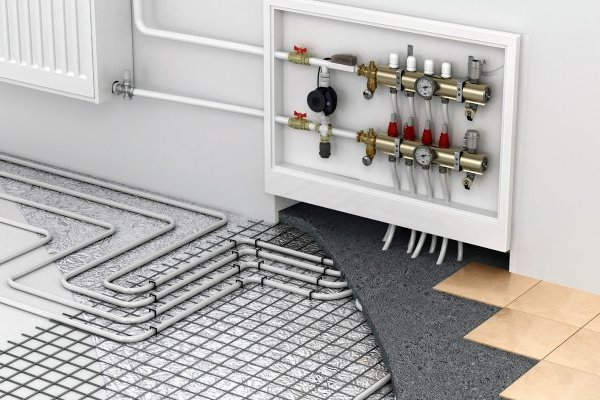
\includegraphics[width=8cm]{Images/suoisan}}
\shortans[oly]{5126}
	\loigiai{
		\begin{itemize}
			\item Ta có: $t_1=22^\circ C, t_2=50^\circ C$
			\item Từ: $Q=mc \Delta t \Rightarrow m=\dfrac{Q}{c \Delta t}=\dfrac{6.10^{8}}{4180.(50-22)}=5126 \ kg$
			\item Vậy bồn cần có 5126 lít nước.
		\end{itemize}
	}
\end{ex}